% Options for packages loaded elsewhere
\PassOptionsToPackage{unicode}{hyperref}
\PassOptionsToPackage{hyphens}{url}
%
\documentclass[
]{article}
\usepackage{amsmath,amssymb}
\usepackage{lmodern}
\usepackage{iftex}
\ifPDFTeX
  \usepackage[T1]{fontenc}
  \usepackage[utf8]{inputenc}
  \usepackage{textcomp} % provide euro and other symbols
\else % if luatex or xetex
  \usepackage{unicode-math}
  \defaultfontfeatures{Scale=MatchLowercase}
  \defaultfontfeatures[\rmfamily]{Ligatures=TeX,Scale=1}
\fi
% Use upquote if available, for straight quotes in verbatim environments
\IfFileExists{upquote.sty}{\usepackage{upquote}}{}
\IfFileExists{microtype.sty}{% use microtype if available
  \usepackage[]{microtype}
  \UseMicrotypeSet[protrusion]{basicmath} % disable protrusion for tt fonts
}{}
\makeatletter
\@ifundefined{KOMAClassName}{% if non-KOMA class
  \IfFileExists{parskip.sty}{%
    \usepackage{parskip}
  }{% else
    \setlength{\parindent}{0pt}
    \setlength{\parskip}{6pt plus 2pt minus 1pt}}
}{% if KOMA class
  \KOMAoptions{parskip=half}}
\makeatother
\usepackage{xcolor}
\usepackage[margin=1in]{geometry}
\usepackage{color}
\usepackage{fancyvrb}
\newcommand{\VerbBar}{|}
\newcommand{\VERB}{\Verb[commandchars=\\\{\}]}
\DefineVerbatimEnvironment{Highlighting}{Verbatim}{commandchars=\\\{\}}
% Add ',fontsize=\small' for more characters per line
\usepackage{framed}
\definecolor{shadecolor}{RGB}{248,248,248}
\newenvironment{Shaded}{\begin{snugshade}}{\end{snugshade}}
\newcommand{\AlertTok}[1]{\textcolor[rgb]{0.94,0.16,0.16}{#1}}
\newcommand{\AnnotationTok}[1]{\textcolor[rgb]{0.56,0.35,0.01}{\textbf{\textit{#1}}}}
\newcommand{\AttributeTok}[1]{\textcolor[rgb]{0.77,0.63,0.00}{#1}}
\newcommand{\BaseNTok}[1]{\textcolor[rgb]{0.00,0.00,0.81}{#1}}
\newcommand{\BuiltInTok}[1]{#1}
\newcommand{\CharTok}[1]{\textcolor[rgb]{0.31,0.60,0.02}{#1}}
\newcommand{\CommentTok}[1]{\textcolor[rgb]{0.56,0.35,0.01}{\textit{#1}}}
\newcommand{\CommentVarTok}[1]{\textcolor[rgb]{0.56,0.35,0.01}{\textbf{\textit{#1}}}}
\newcommand{\ConstantTok}[1]{\textcolor[rgb]{0.00,0.00,0.00}{#1}}
\newcommand{\ControlFlowTok}[1]{\textcolor[rgb]{0.13,0.29,0.53}{\textbf{#1}}}
\newcommand{\DataTypeTok}[1]{\textcolor[rgb]{0.13,0.29,0.53}{#1}}
\newcommand{\DecValTok}[1]{\textcolor[rgb]{0.00,0.00,0.81}{#1}}
\newcommand{\DocumentationTok}[1]{\textcolor[rgb]{0.56,0.35,0.01}{\textbf{\textit{#1}}}}
\newcommand{\ErrorTok}[1]{\textcolor[rgb]{0.64,0.00,0.00}{\textbf{#1}}}
\newcommand{\ExtensionTok}[1]{#1}
\newcommand{\FloatTok}[1]{\textcolor[rgb]{0.00,0.00,0.81}{#1}}
\newcommand{\FunctionTok}[1]{\textcolor[rgb]{0.00,0.00,0.00}{#1}}
\newcommand{\ImportTok}[1]{#1}
\newcommand{\InformationTok}[1]{\textcolor[rgb]{0.56,0.35,0.01}{\textbf{\textit{#1}}}}
\newcommand{\KeywordTok}[1]{\textcolor[rgb]{0.13,0.29,0.53}{\textbf{#1}}}
\newcommand{\NormalTok}[1]{#1}
\newcommand{\OperatorTok}[1]{\textcolor[rgb]{0.81,0.36,0.00}{\textbf{#1}}}
\newcommand{\OtherTok}[1]{\textcolor[rgb]{0.56,0.35,0.01}{#1}}
\newcommand{\PreprocessorTok}[1]{\textcolor[rgb]{0.56,0.35,0.01}{\textit{#1}}}
\newcommand{\RegionMarkerTok}[1]{#1}
\newcommand{\SpecialCharTok}[1]{\textcolor[rgb]{0.00,0.00,0.00}{#1}}
\newcommand{\SpecialStringTok}[1]{\textcolor[rgb]{0.31,0.60,0.02}{#1}}
\newcommand{\StringTok}[1]{\textcolor[rgb]{0.31,0.60,0.02}{#1}}
\newcommand{\VariableTok}[1]{\textcolor[rgb]{0.00,0.00,0.00}{#1}}
\newcommand{\VerbatimStringTok}[1]{\textcolor[rgb]{0.31,0.60,0.02}{#1}}
\newcommand{\WarningTok}[1]{\textcolor[rgb]{0.56,0.35,0.01}{\textbf{\textit{#1}}}}
\usepackage{longtable,booktabs,array}
\usepackage{calc} % for calculating minipage widths
% Correct order of tables after \paragraph or \subparagraph
\usepackage{etoolbox}
\makeatletter
\patchcmd\longtable{\par}{\if@noskipsec\mbox{}\fi\par}{}{}
\makeatother
% Allow footnotes in longtable head/foot
\IfFileExists{footnotehyper.sty}{\usepackage{footnotehyper}}{\usepackage{footnote}}
\makesavenoteenv{longtable}
\usepackage{graphicx}
\makeatletter
\def\maxwidth{\ifdim\Gin@nat@width>\linewidth\linewidth\else\Gin@nat@width\fi}
\def\maxheight{\ifdim\Gin@nat@height>\textheight\textheight\else\Gin@nat@height\fi}
\makeatother
% Scale images if necessary, so that they will not overflow the page
% margins by default, and it is still possible to overwrite the defaults
% using explicit options in \includegraphics[width, height, ...]{}
\setkeys{Gin}{width=\maxwidth,height=\maxheight,keepaspectratio}
% Set default figure placement to htbp
\makeatletter
\def\fps@figure{htbp}
\makeatother
\setlength{\emergencystretch}{3em} % prevent overfull lines
\providecommand{\tightlist}{%
  \setlength{\itemsep}{0pt}\setlength{\parskip}{0pt}}
\setcounter{secnumdepth}{-\maxdimen} % remove section numbering
\ifLuaTeX
  \usepackage{selnolig}  % disable illegal ligatures
\fi
\IfFileExists{bookmark.sty}{\usepackage{bookmark}}{\usepackage{hyperref}}
\IfFileExists{xurl.sty}{\usepackage{xurl}}{} % add URL line breaks if available
\urlstyle{same} % disable monospaced font for URLs
\hypersetup{
  pdftitle={Genetic differentiation on flowering time in Cerastium fontanum using a greenhouse experiment},
  pdfauthor={Alicia Valdés},
  hidelinks,
  pdfcreator={LaTeX via pandoc}}

\title{Genetic differentiation on flowering time in Cerastium fontanum
using a greenhouse experiment}
\usepackage{etoolbox}
\makeatletter
\providecommand{\subtitle}[1]{% add subtitle to \maketitle
  \apptocmd{\@title}{\par {\large #1 \par}}{}{}
}
\makeatother
\subtitle{Data preparation and first analyses}
\author{Alicia Valdés}
\date{02 March, 2023}

\begin{document}
\maketitle

{
\setcounter{tocdepth}{4}
\tableofcontents
}
\hypertarget{data-preparation}{%
\section{Data preparation}\label{data-preparation}}

\hypertarget{read-data-from-excel-files}{%
\subsection{Read data from Excel
files}\label{read-data-from-excel-files}}

\begin{Shaded}
\begin{Highlighting}[]
\NormalTok{data\_exp}\OtherTok{\textless{}{-}}\FunctionTok{read\_excel}\NormalTok{(}\StringTok{"data/edited/Cerastium\_greenhouse\_spring\_2022.xlsx"}\NormalTok{, }
                       \AttributeTok{sheet=}\StringTok{"extracted\_data"}\NormalTok{)}
\NormalTok{data\_exp}\SpecialCharTok{$}\NormalTok{treat}\OtherTok{\textless{}{-}}\FunctionTok{as.factor}\NormalTok{(data\_exp}\SpecialCharTok{$}\NormalTok{treat)}
\NormalTok{data\_exp}\SpecialCharTok{$}\NormalTok{mother}\OtherTok{\textless{}{-}}\FunctionTok{as.factor}\NormalTok{(data\_exp}\SpecialCharTok{$}\NormalTok{mother)}
\NormalTok{data\_exp}\SpecialCharTok{$}\NormalTok{father}\OtherTok{\textless{}{-}}\FunctionTok{as.factor}\NormalTok{(data\_exp}\SpecialCharTok{$}\NormalTok{father)}
\NormalTok{data\_exp}\SpecialCharTok{$}\NormalTok{total\_n\_fl}\OtherTok{\textless{}{-}}\FunctionTok{as.integer}\NormalTok{(data\_exp}\SpecialCharTok{$}\NormalTok{total\_n\_fl)}
\NormalTok{data\_exp}\SpecialCharTok{$}\NormalTok{date50}\OtherTok{\textless{}{-}}\FunctionTok{as.numeric}\NormalTok{(data\_exp}\SpecialCharTok{$}\NormalTok{date50)}
\end{Highlighting}
\end{Shaded}

\begin{Shaded}
\begin{Highlighting}[]
\NormalTok{data\_parents}\OtherTok{\textless{}{-}}\FunctionTok{read\_excel}\NormalTok{(}\StringTok{"data/edited/Cerastium\_greenhouse\_spring\_2022.xlsx"}\NormalTok{, }
                       \AttributeTok{sheet=}\StringTok{"extracted\_data\_parents"}\NormalTok{)}
\NormalTok{data\_parents}\SpecialCharTok{$}\NormalTok{treat}\OtherTok{\textless{}{-}}\FunctionTok{as.factor}\NormalTok{(data\_parents}\SpecialCharTok{$}\NormalTok{treat)}
\end{Highlighting}
\end{Shaded}

\begin{Shaded}
\begin{Highlighting}[]
\FunctionTok{head}\NormalTok{(data\_exp)}
\end{Highlighting}
\end{Shaded}

\begin{verbatim}
## # A tibble: 6 x 10
##   mother father temp_mother temp_father treat    total_n_fl   FFD   LFD date50
##   <fct>  <fct>        <dbl>       <dbl> <fct>         <int> <dbl> <dbl>  <dbl>
## 1 16     120           25.9        11.3 unheated         13   129   154    138
## 2 39     350           22.6        20.6 unheated          0    NA    NA     NA
## 3 26     250           21.5        23.4 unheated          6   124   140    129
## 4 31     310            7           8   unheated         64   115   150    128
## 5 24     210           14.9         7   unheated          6   124   145    129
## 6 34     320           18           9   unheated         15   129   161    138
##   Comments
##   <chr>   
## 1 <NA>    
## 2 <NA>    
## 3 <NA>    
## 4 <NA>    
## 5 <NA>    
## 6 <NA>
\end{verbatim}

\begin{Shaded}
\begin{Highlighting}[]
\FunctionTok{head}\NormalTok{(data\_parents)}
\end{Highlighting}
\end{Shaded}

\begin{verbatim}
## # A tibble: 6 x 7
##    temp treat    total_n_fl   FFD   LFD date50 Comments
##   <dbl> <fct>         <dbl> <dbl> <dbl>  <dbl> <chr>   
## 1  11.3 unheated         17   124   143    134 <NA>    
## 2   9   unheated          0    NA    NA     NA <NA>    
## 3  23.4 unheated          8   124   140    128 <NA>    
## 4  20.6 unheated          0    NA    NA     NA <NA>    
## 5  21.6 unheated         24   122   154    132 <NA>    
## 6  45.5 unheated         12   124   150    131 <NA>
\end{verbatim}

\hypertarget{how-many-different-mothers-and-fathers}{%
\subsection{How many different mothers and
fathers?}\label{how-many-different-mothers-and-fathers}}

\begin{Shaded}
\begin{Highlighting}[]
\FunctionTok{length}\NormalTok{(}\FunctionTok{levels}\NormalTok{(data\_exp}\SpecialCharTok{$}\NormalTok{mother)) }\CommentTok{\# 25 different mothers (shouldn\textquotesingle{}t it be 24?)}
\end{Highlighting}
\end{Shaded}

\begin{verbatim}
## [1] 25
\end{verbatim}

\begin{Shaded}
\begin{Highlighting}[]
\FunctionTok{length}\NormalTok{(}\FunctionTok{levels}\NormalTok{(data\_exp}\SpecialCharTok{$}\NormalTok{father)) }\CommentTok{\# 24 different mothers}
\end{Highlighting}
\end{Shaded}

\begin{verbatim}
## [1] 24
\end{verbatim}

\hypertarget{how-many-unique-combinations-of-mothers-and-fathers}{%
\subsection{How many unique combinations of mothers and
fathers?}\label{how-many-unique-combinations-of-mothers-and-fathers}}

\begin{Shaded}
\begin{Highlighting}[]
\NormalTok{data\_exp}\OtherTok{\textless{}{-}}\NormalTok{data\_exp}\SpecialCharTok{\%\textgreater{}\%}\FunctionTok{mutate}\NormalTok{(}\AttributeTok{mother\_father=}\FunctionTok{paste}\NormalTok{(mother,father,}\AttributeTok{sep=}\StringTok{"\_"}\NormalTok{))}
\end{Highlighting}
\end{Shaded}

\begin{Shaded}
\begin{Highlighting}[]
\FunctionTok{length}\NormalTok{(}\FunctionTok{unique}\NormalTok{(data\_exp}\SpecialCharTok{$}\NormalTok{mother\_father)) }\CommentTok{\# 100 (shouldn\textquotesingle{}t it be 96?)}
\end{Highlighting}
\end{Shaded}

\begin{verbatim}
## [1] 100
\end{verbatim}

\begin{Shaded}
\begin{Highlighting}[]
\CommentTok{\# It is really 99, because one is "NA\_NA"}
\end{Highlighting}
\end{Shaded}

\hypertarget{number-of-plants-from-each-crossing}{%
\subsection{Number of plants from each
crossing}\label{number-of-plants-from-each-crossing}}

\begin{Shaded}
\begin{Highlighting}[]
\NormalTok{data\_exp}\SpecialCharTok{\%\textgreater{}\%}\FunctionTok{group\_by}\NormalTok{(mother\_father)}\SpecialCharTok{\%\textgreater{}\%}\FunctionTok{summarise}\NormalTok{(}\AttributeTok{num=}\FunctionTok{n}\NormalTok{())}\SpecialCharTok{\%\textgreater{}\%}
  \FunctionTok{ggplot}\NormalTok{(}\FunctionTok{aes}\NormalTok{(}\AttributeTok{x=}\NormalTok{num))}\SpecialCharTok{+}\FunctionTok{geom\_histogram}\NormalTok{(}\AttributeTok{bins=}\DecValTok{12}\NormalTok{)}
\end{Highlighting}
\end{Shaded}

\includegraphics{1_data_prep_analyses_files/figure-latex/unnamed-chunk-7-1.pdf}

12 plants from most crossings, but also one with 13 and some with fewer.

\hypertarget{distributions}{%
\section{Distributions}\label{distributions}}

\begin{Shaded}
\begin{Highlighting}[]
\FunctionTok{hist}\NormalTok{(data\_exp}\SpecialCharTok{$}\NormalTok{FFD)}
\end{Highlighting}
\end{Shaded}

\includegraphics{1_data_prep_analyses_files/figure-latex/unnamed-chunk-8-1.pdf}

\begin{Shaded}
\begin{Highlighting}[]
\FunctionTok{hist}\NormalTok{(data\_exp}\SpecialCharTok{$}\NormalTok{LFD)}
\end{Highlighting}
\end{Shaded}

\includegraphics{1_data_prep_analyses_files/figure-latex/unnamed-chunk-8-2.pdf}

\begin{Shaded}
\begin{Highlighting}[]
\FunctionTok{hist}\NormalTok{(data\_exp}\SpecialCharTok{$}\NormalTok{date50)}
\end{Highlighting}
\end{Shaded}

\includegraphics{1_data_prep_analyses_files/figure-latex/unnamed-chunk-8-3.pdf}

All looking quite normal.

\hypertarget{analyses}{%
\section{Analyses}\label{analyses}}

\hypertarget{with-offspring-from-crosses}{%
\subsection{With offspring from
crosses}\label{with-offspring-from-crosses}}

\begin{Shaded}
\begin{Highlighting}[]
\NormalTok{model\_offpsring\_FFD}\OtherTok{\textless{}{-}}\FunctionTok{glmmTMB}\NormalTok{(FFD}\SpecialCharTok{\textasciitilde{}}\NormalTok{(temp\_mother}\SpecialCharTok{+}\NormalTok{temp\_father)}\SpecialCharTok{*}\NormalTok{treat}\SpecialCharTok{+}
\NormalTok{                               (}\DecValTok{1}\SpecialCharTok{|}\NormalTok{mother)}\SpecialCharTok{+}\NormalTok{(}\DecValTok{1}\SpecialCharTok{|}\NormalTok{father),data\_exp)}
\NormalTok{model\_offpsring\_LFD}\OtherTok{\textless{}{-}}\FunctionTok{glmmTMB}\NormalTok{(LFD}\SpecialCharTok{\textasciitilde{}}\NormalTok{(temp\_mother}\SpecialCharTok{+}\NormalTok{temp\_father)}\SpecialCharTok{*}\NormalTok{treat}\SpecialCharTok{+}
\NormalTok{                               (}\DecValTok{1}\SpecialCharTok{|}\NormalTok{mother)}\SpecialCharTok{+}\NormalTok{(}\DecValTok{1}\SpecialCharTok{|}\NormalTok{father),data\_exp)}
\NormalTok{model\_offpsring\_date50}\OtherTok{\textless{}{-}}\FunctionTok{glmmTMB}\NormalTok{(date50}\SpecialCharTok{\textasciitilde{}}\NormalTok{(temp\_mother}\SpecialCharTok{+}\NormalTok{temp\_father)}\SpecialCharTok{*}\NormalTok{treat}\SpecialCharTok{+}
\NormalTok{                               (}\DecValTok{1}\SpecialCharTok{|}\NormalTok{mother)}\SpecialCharTok{+}\NormalTok{(}\DecValTok{1}\SpecialCharTok{|}\NormalTok{father),data\_exp)}
\FunctionTok{kable}\NormalTok{(}\FunctionTok{tidy}\NormalTok{(model\_offpsring\_FFD),}\AttributeTok{digits=}\FunctionTok{c}\NormalTok{(}\DecValTok{3}\NormalTok{,}\DecValTok{3}\NormalTok{,}\DecValTok{2}\NormalTok{,}\DecValTok{3}\NormalTok{))}
\end{Highlighting}
\end{Shaded}

\begin{longtable}[]{@{}
  >{\raggedright\arraybackslash}p{(\columnwidth - 14\tabcolsep) * \real{0.0989}}
  >{\raggedright\arraybackslash}p{(\columnwidth - 14\tabcolsep) * \real{0.1099}}
  >{\raggedright\arraybackslash}p{(\columnwidth - 14\tabcolsep) * \real{0.0989}}
  >{\raggedright\arraybackslash}p{(\columnwidth - 14\tabcolsep) * \real{0.2857}}
  >{\raggedleft\arraybackslash}p{(\columnwidth - 14\tabcolsep) * \real{0.0989}}
  >{\raggedleft\arraybackslash}p{(\columnwidth - 14\tabcolsep) * \real{0.1099}}
  >{\raggedleft\arraybackslash}p{(\columnwidth - 14\tabcolsep) * \real{0.1099}}
  >{\raggedleft\arraybackslash}p{(\columnwidth - 14\tabcolsep) * \real{0.0879}}@{}}
\toprule()
\begin{minipage}[b]{\linewidth}\raggedright
effect
\end{minipage} & \begin{minipage}[b]{\linewidth}\raggedright
component
\end{minipage} & \begin{minipage}[b]{\linewidth}\raggedright
group
\end{minipage} & \begin{minipage}[b]{\linewidth}\raggedright
term
\end{minipage} & \begin{minipage}[b]{\linewidth}\raggedleft
estimate
\end{minipage} & \begin{minipage}[b]{\linewidth}\raggedleft
std.error
\end{minipage} & \begin{minipage}[b]{\linewidth}\raggedleft
statistic
\end{minipage} & \begin{minipage}[b]{\linewidth}\raggedleft
p.value
\end{minipage} \\
\midrule()
\endhead
fixed & cond & NA & (Intercept) & 119.755 & 2.184 & 54.83 & 0.000 \\
fixed & cond & NA & temp\_mother & -0.015 & 0.094 & -0.16 & 0.873 \\
fixed & cond & NA & temp\_father & 0.029 & 0.050 & 0.57 & 0.569 \\
fixed & cond & NA & treatunheated & 9.079 & 1.466 & 6.19 & 0.000 \\
fixed & cond & NA & temp\_mother:treatunheated & 0.008 & 0.059 & 0.13 &
0.896 \\
fixed & cond & NA & temp\_father:treatunheated & 0.008 & 0.043 & 0.20 &
0.842 \\
ran\_pars & cond & mother & sd\_\_(Intercept) & 3.367 & NA & NA & NA \\
ran\_pars & cond & father & sd\_\_(Intercept) & 2.033 & NA & NA & NA \\
ran\_pars & cond & Residual & sd\_\_Observation & 7.006 & NA & NA &
NA \\
\bottomrule()
\end{longtable}

\begin{Shaded}
\begin{Highlighting}[]
\FunctionTok{kable}\NormalTok{(}\FunctionTok{tidy}\NormalTok{(model\_offpsring\_LFD),}\AttributeTok{digits=}\FunctionTok{c}\NormalTok{(}\DecValTok{3}\NormalTok{,}\DecValTok{3}\NormalTok{,}\DecValTok{2}\NormalTok{,}\DecValTok{3}\NormalTok{))}
\end{Highlighting}
\end{Shaded}

\begin{longtable}[]{@{}
  >{\raggedright\arraybackslash}p{(\columnwidth - 14\tabcolsep) * \real{0.0989}}
  >{\raggedright\arraybackslash}p{(\columnwidth - 14\tabcolsep) * \real{0.1099}}
  >{\raggedright\arraybackslash}p{(\columnwidth - 14\tabcolsep) * \real{0.0989}}
  >{\raggedright\arraybackslash}p{(\columnwidth - 14\tabcolsep) * \real{0.2857}}
  >{\raggedleft\arraybackslash}p{(\columnwidth - 14\tabcolsep) * \real{0.0989}}
  >{\raggedleft\arraybackslash}p{(\columnwidth - 14\tabcolsep) * \real{0.1099}}
  >{\raggedleft\arraybackslash}p{(\columnwidth - 14\tabcolsep) * \real{0.1099}}
  >{\raggedleft\arraybackslash}p{(\columnwidth - 14\tabcolsep) * \real{0.0879}}@{}}
\toprule()
\begin{minipage}[b]{\linewidth}\raggedright
effect
\end{minipage} & \begin{minipage}[b]{\linewidth}\raggedright
component
\end{minipage} & \begin{minipage}[b]{\linewidth}\raggedright
group
\end{minipage} & \begin{minipage}[b]{\linewidth}\raggedright
term
\end{minipage} & \begin{minipage}[b]{\linewidth}\raggedleft
estimate
\end{minipage} & \begin{minipage}[b]{\linewidth}\raggedleft
std.error
\end{minipage} & \begin{minipage}[b]{\linewidth}\raggedleft
statistic
\end{minipage} & \begin{minipage}[b]{\linewidth}\raggedleft
p.value
\end{minipage} \\
\midrule()
\endhead
fixed & cond & NA & (Intercept) & 135.570 & 1.981 & 68.45 & 0.000 \\
fixed & cond & NA & temp\_mother & 0.075 & 0.084 & 0.88 & 0.377 \\
fixed & cond & NA & temp\_father & 0.059 & 0.049 & 1.20 & 0.230 \\
fixed & cond & NA & treatunheated & 9.998 & 1.847 & 5.41 & 0.000 \\
fixed & cond & NA & temp\_mother:treatunheated & 0.056 & 0.075 & 0.74 &
0.458 \\
fixed & cond & NA & temp\_father:treatunheated & -0.012 & 0.054 & -0.22
& 0.825 \\
ran\_pars & cond & mother & sd\_\_(Intercept) & 2.604 & NA & NA & NA \\
ran\_pars & cond & father & sd\_\_(Intercept) & 1.506 & NA & NA & NA \\
ran\_pars & cond & Residual & sd\_\_Observation & 8.843 & NA & NA &
NA \\
\bottomrule()
\end{longtable}

\begin{Shaded}
\begin{Highlighting}[]
\FunctionTok{kable}\NormalTok{(}\FunctionTok{tidy}\NormalTok{(model\_offpsring\_date50),}\AttributeTok{digits=}\FunctionTok{c}\NormalTok{(}\DecValTok{3}\NormalTok{,}\DecValTok{3}\NormalTok{,}\DecValTok{2}\NormalTok{,}\DecValTok{3}\NormalTok{))}
\end{Highlighting}
\end{Shaded}

\begin{longtable}[]{@{}
  >{\raggedright\arraybackslash}p{(\columnwidth - 14\tabcolsep) * \real{0.0989}}
  >{\raggedright\arraybackslash}p{(\columnwidth - 14\tabcolsep) * \real{0.1099}}
  >{\raggedright\arraybackslash}p{(\columnwidth - 14\tabcolsep) * \real{0.0989}}
  >{\raggedright\arraybackslash}p{(\columnwidth - 14\tabcolsep) * \real{0.2857}}
  >{\raggedleft\arraybackslash}p{(\columnwidth - 14\tabcolsep) * \real{0.0989}}
  >{\raggedleft\arraybackslash}p{(\columnwidth - 14\tabcolsep) * \real{0.1099}}
  >{\raggedleft\arraybackslash}p{(\columnwidth - 14\tabcolsep) * \real{0.1099}}
  >{\raggedleft\arraybackslash}p{(\columnwidth - 14\tabcolsep) * \real{0.0879}}@{}}
\toprule()
\begin{minipage}[b]{\linewidth}\raggedright
effect
\end{minipage} & \begin{minipage}[b]{\linewidth}\raggedright
component
\end{minipage} & \begin{minipage}[b]{\linewidth}\raggedright
group
\end{minipage} & \begin{minipage}[b]{\linewidth}\raggedright
term
\end{minipage} & \begin{minipage}[b]{\linewidth}\raggedleft
estimate
\end{minipage} & \begin{minipage}[b]{\linewidth}\raggedleft
std.error
\end{minipage} & \begin{minipage}[b]{\linewidth}\raggedleft
statistic
\end{minipage} & \begin{minipage}[b]{\linewidth}\raggedleft
p.value
\end{minipage} \\
\midrule()
\endhead
fixed & cond & NA & (Intercept) & 123.564 & 1.821 & 67.86 & 0.000 \\
fixed & cond & NA & temp\_mother & 0.076 & 0.081 & 0.93 & 0.353 \\
fixed & cond & NA & temp\_father & 0.083 & 0.037 & 2.27 & 0.023 \\
fixed & cond & NA & treatunheated & 9.853 & 1.237 & 7.96 & 0.000 \\
fixed & cond & NA & temp\_mother:treatunheated & 0.008 & 0.050 & 0.15 &
0.877 \\
fixed & cond & NA & temp\_father:treatunheated & -0.030 & 0.036 & -0.84
& 0.399 \\
ran\_pars & cond & mother & sd\_\_(Intercept) & 2.946 & NA & NA & NA \\
ran\_pars & cond & father & sd\_\_(Intercept) & 1.303 & NA & NA & NA \\
ran\_pars & cond & Residual & sd\_\_Observation & 5.921 & NA & NA &
NA \\
\bottomrule()
\end{longtable}

Only effects of treatment are significant for FFD and LFD, also
temp\_father for date 50.

Save models as HTML table

\begin{Shaded}
\begin{Highlighting}[]
\FunctionTok{tab\_model}\NormalTok{(model\_offpsring\_FFD,model\_offpsring\_LFD,model\_offpsring\_date50,}
          \AttributeTok{transform=}\ConstantTok{NULL}\NormalTok{,}\AttributeTok{show.ci=}\NormalTok{F,}\AttributeTok{show.se=}\NormalTok{T,}\AttributeTok{show.stat=}\NormalTok{T,}\AttributeTok{digits=}\DecValTok{3}\NormalTok{,}
          \AttributeTok{dv.labels=}\FunctionTok{c}\NormalTok{(}\StringTok{"FFD"}\NormalTok{,}\StringTok{"LFD"}\NormalTok{,}\StringTok{"date50"}\NormalTok{),}
          \AttributeTok{file=}\StringTok{"output/tables/Table\_models\_offspring.html"}\NormalTok{,}
          \AttributeTok{title=}\StringTok{"Models offspring"}\NormalTok{)}
\end{Highlighting}
\end{Shaded}

Models offspring

~

FFD

LFD

date50

Predictors

Estimates

std. Error

Statistic

p

Estimates

std. Error

Statistic

p

Estimates

std. Error

Statistic

p

(Intercept)

119.755

2.184

54.828

\textless0.001

135.570

1.981

68.449

\textless0.001

123.564

1.821

67.855

\textless0.001

temp mother

-0.015

0.094

-0.160

0.873

0.075

0.084

0.883

0.377

0.076

0.081

0.929

0.353

temp father

0.029

0.050

0.570

0.569

0.059

0.049

1.202

0.230

0.083

0.037

2.267

0.023

treat {[}unheated{]}

9.079

1.466

6.193

\textless0.001

9.998

1.847

5.414

\textless0.001

9.853

1.237

7.964

\textless0.001

temp mother × treat{[}unheated{]}

0.008

0.059

0.130

0.896

0.056

0.075

0.742

0.458

0.008

0.050

0.155

0.877

temp father × treat{[}unheated{]}

0.008

0.043

0.199

0.842

-0.012

0.054

-0.221

0.825

-0.030

0.036

-0.843

0.399

Random Effects

σ2

49.08

78.21

35.06

τ00

11.34 mother

6.78 mother

8.68 mother

4.13 father

2.27 father

1.70 father

ICC

0.24

0.10

0.23

N

25 mother

25 mother

25 mother

24 father

24 father

24 father

Observations

844

845

845

Marginal R2 / Conditional R2

0.257 / 0.435

0.258 / 0.335

0.337 / 0.488

Plot predictions of significant effects

\begin{Shaded}
\begin{Highlighting}[]
\FunctionTok{plot}\NormalTok{(}\FunctionTok{ggpredict}\NormalTok{(model\_offpsring\_FFD,}\AttributeTok{terms=}\FunctionTok{c}\NormalTok{(}\StringTok{"treat"}\NormalTok{)))}
\end{Highlighting}
\end{Shaded}

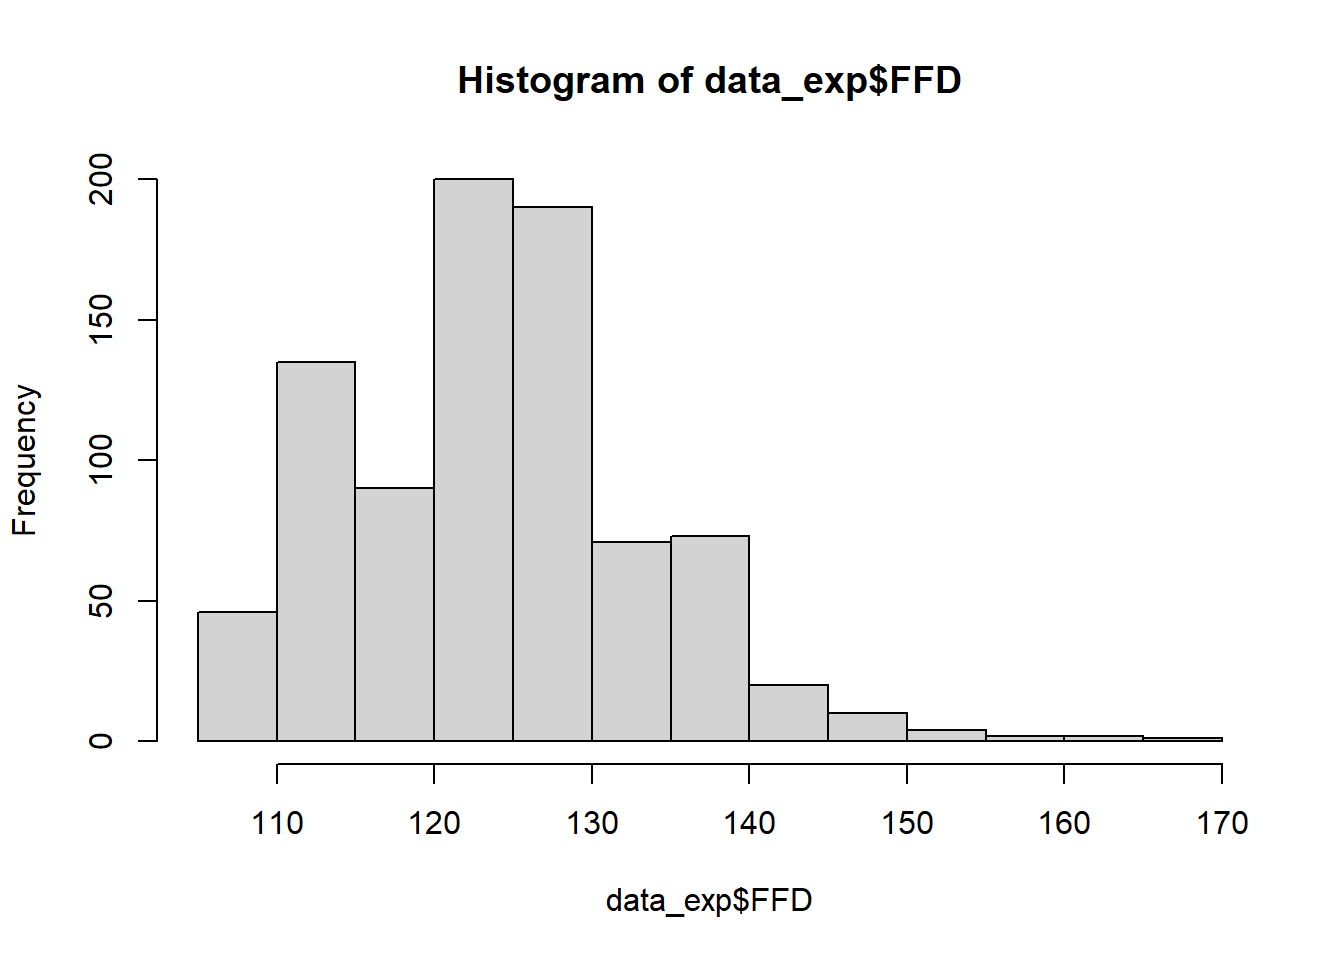
\includegraphics{1_data_prep_analyses_files/figure-latex/unnamed-chunk-11-1.pdf}

\begin{Shaded}
\begin{Highlighting}[]
\FunctionTok{plot}\NormalTok{(}\FunctionTok{ggpredict}\NormalTok{(model\_offpsring\_LFD,}\AttributeTok{terms=}\FunctionTok{c}\NormalTok{(}\StringTok{"treat"}\NormalTok{)))}
\end{Highlighting}
\end{Shaded}

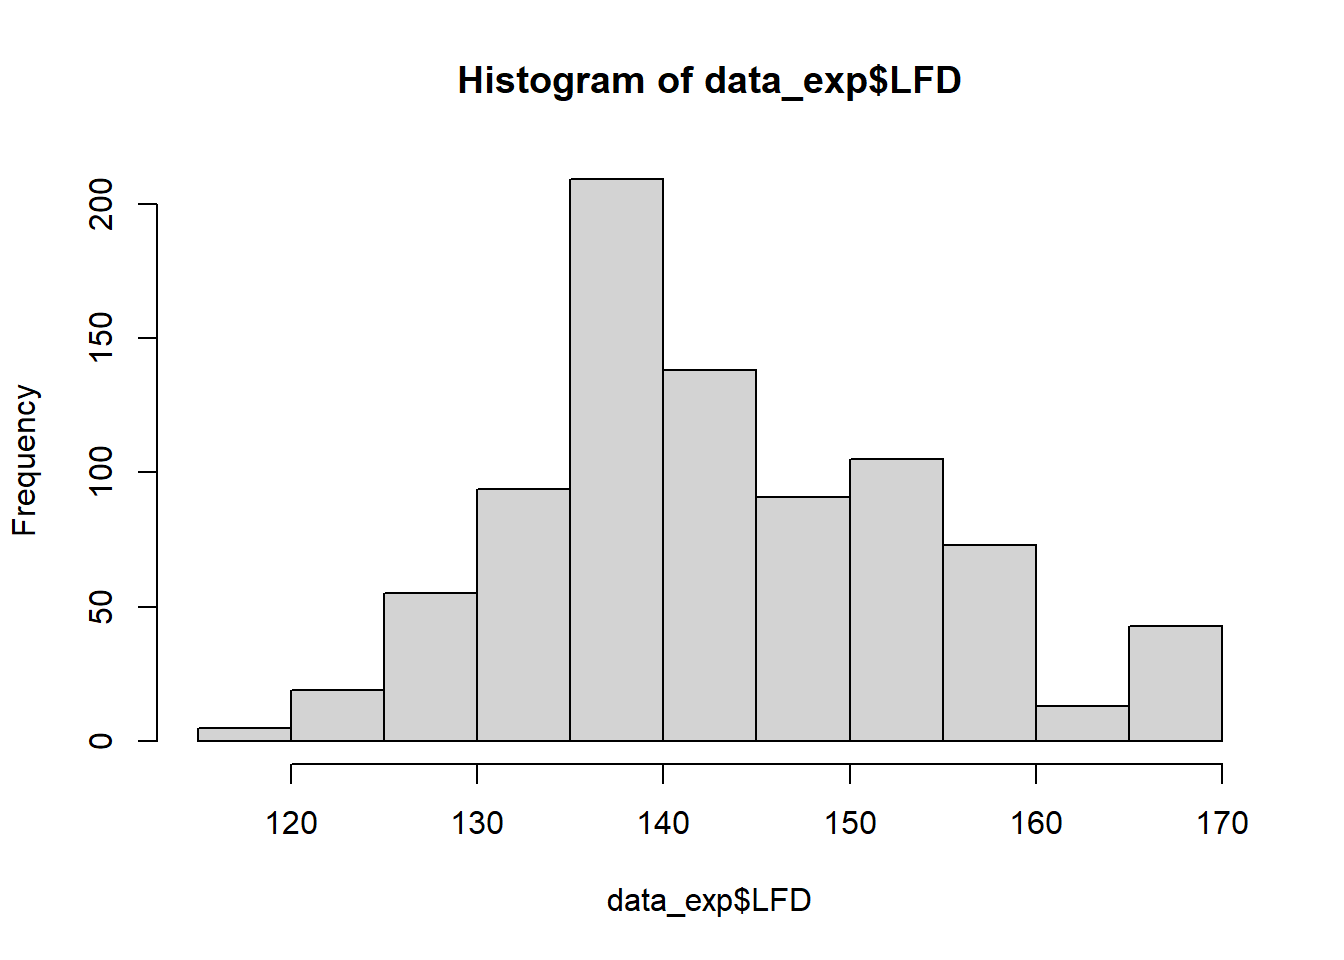
\includegraphics{1_data_prep_analyses_files/figure-latex/unnamed-chunk-11-2.pdf}

\begin{Shaded}
\begin{Highlighting}[]
\FunctionTok{plot}\NormalTok{(}\FunctionTok{ggpredict}\NormalTok{(model\_offpsring\_date50,}\AttributeTok{terms=}\FunctionTok{c}\NormalTok{(}\StringTok{"treat"}\NormalTok{)))}
\end{Highlighting}
\end{Shaded}

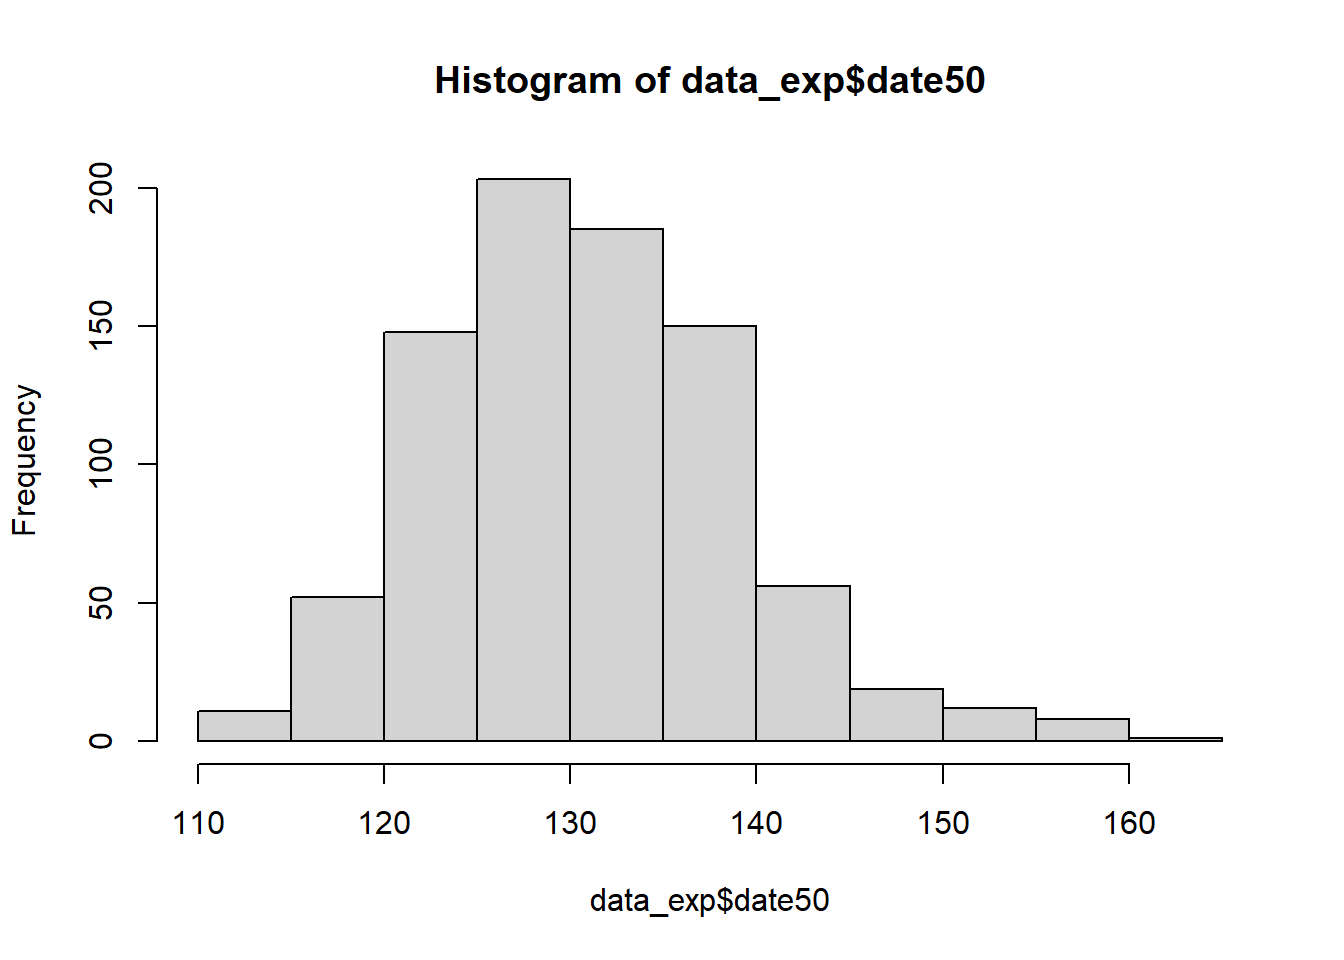
\includegraphics{1_data_prep_analyses_files/figure-latex/unnamed-chunk-11-3.pdf}

\begin{Shaded}
\begin{Highlighting}[]
\FunctionTok{plot}\NormalTok{(}\FunctionTok{ggpredict}\NormalTok{(model\_offpsring\_date50,}\AttributeTok{terms=}\FunctionTok{c}\NormalTok{(}\StringTok{"temp\_father"}\NormalTok{)))}
\end{Highlighting}
\end{Shaded}

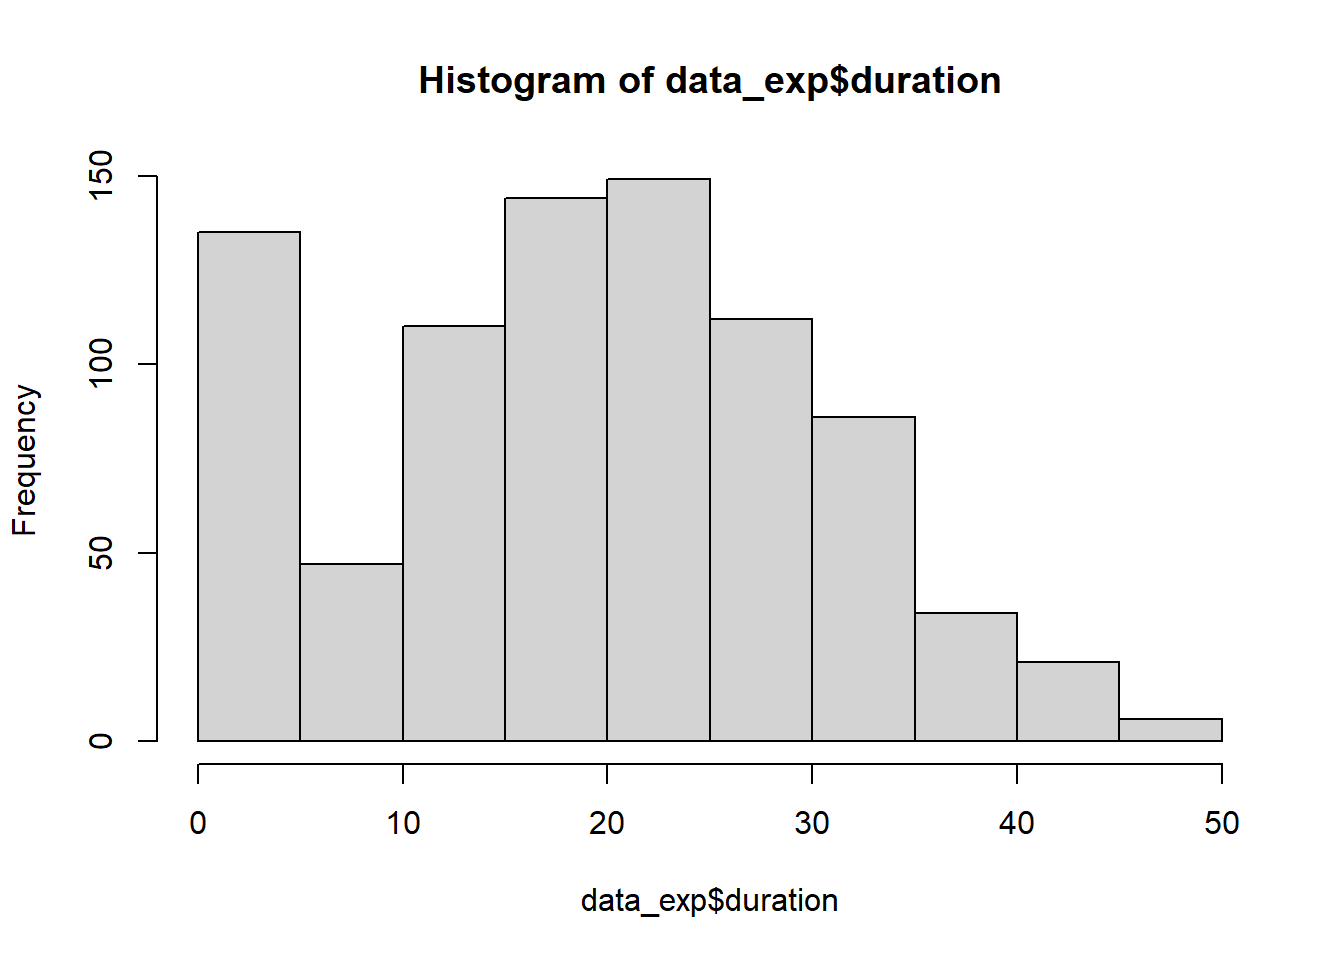
\includegraphics{1_data_prep_analyses_files/figure-latex/unnamed-chunk-11-4.pdf}

Plot predictions of interactions (NS)

\begin{Shaded}
\begin{Highlighting}[]
\FunctionTok{plot}\NormalTok{(}\FunctionTok{ggpredict}\NormalTok{(model\_offpsring\_FFD,}\AttributeTok{terms=}\FunctionTok{c}\NormalTok{(}\StringTok{"temp\_mother"}\NormalTok{,}\StringTok{"treat"}\NormalTok{)))}
\end{Highlighting}
\end{Shaded}

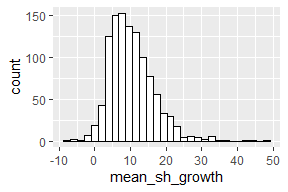
\includegraphics{1_data_prep_analyses_files/figure-latex/unnamed-chunk-12-1.pdf}

\begin{Shaded}
\begin{Highlighting}[]
\FunctionTok{plot}\NormalTok{(}\FunctionTok{ggpredict}\NormalTok{(model\_offpsring\_LFD,}\AttributeTok{terms=}\FunctionTok{c}\NormalTok{(}\StringTok{"temp\_mother"}\NormalTok{,}\StringTok{"treat"}\NormalTok{)))}
\end{Highlighting}
\end{Shaded}

\includegraphics{1_data_prep_analyses_files/figure-latex/unnamed-chunk-12-2.pdf}

\begin{Shaded}
\begin{Highlighting}[]
\FunctionTok{plot}\NormalTok{(}\FunctionTok{ggpredict}\NormalTok{(model\_offpsring\_date50,}\AttributeTok{terms=}\FunctionTok{c}\NormalTok{(}\StringTok{"temp\_mother"}\NormalTok{,}\StringTok{"treat"}\NormalTok{)))}
\end{Highlighting}
\end{Shaded}

\includegraphics{1_data_prep_analyses_files/figure-latex/unnamed-chunk-12-3.pdf}

\begin{Shaded}
\begin{Highlighting}[]
\FunctionTok{plot}\NormalTok{(}\FunctionTok{ggpredict}\NormalTok{(model\_offpsring\_FFD,}\AttributeTok{terms=}\FunctionTok{c}\NormalTok{(}\StringTok{"temp\_father"}\NormalTok{,}\StringTok{"treat"}\NormalTok{)))}
\end{Highlighting}
\end{Shaded}

\includegraphics{1_data_prep_analyses_files/figure-latex/unnamed-chunk-12-4.pdf}

\begin{Shaded}
\begin{Highlighting}[]
\FunctionTok{plot}\NormalTok{(}\FunctionTok{ggpredict}\NormalTok{(model\_offpsring\_LFD,}\AttributeTok{terms=}\FunctionTok{c}\NormalTok{(}\StringTok{"temp\_father"}\NormalTok{,}\StringTok{"treat"}\NormalTok{)))}
\end{Highlighting}
\end{Shaded}

\includegraphics{1_data_prep_analyses_files/figure-latex/unnamed-chunk-12-5.pdf}

\begin{Shaded}
\begin{Highlighting}[]
\FunctionTok{plot}\NormalTok{(}\FunctionTok{ggpredict}\NormalTok{(model\_offpsring\_date50,}\AttributeTok{terms=}\FunctionTok{c}\NormalTok{(}\StringTok{"temp\_father"}\NormalTok{,}\StringTok{"treat"}\NormalTok{)))}
\end{Highlighting}
\end{Shaded}

\includegraphics{1_data_prep_analyses_files/figure-latex/unnamed-chunk-12-6.pdf}

\hypertarget{with-parents}{%
\subsection{With parents}\label{with-parents}}

\begin{Shaded}
\begin{Highlighting}[]
\NormalTok{model\_parents\_FFD}\OtherTok{\textless{}{-}}\FunctionTok{lm}\NormalTok{(FFD}\SpecialCharTok{\textasciitilde{}}\NormalTok{temp}\SpecialCharTok{*}\NormalTok{treat,data\_parents)}
\NormalTok{model\_parents\_LFD}\OtherTok{\textless{}{-}}\FunctionTok{lm}\NormalTok{(LFD}\SpecialCharTok{\textasciitilde{}}\NormalTok{temp}\SpecialCharTok{*}\NormalTok{treat,data\_parents)}
\NormalTok{model\_parents\_date50}\OtherTok{\textless{}{-}}\FunctionTok{lm}\NormalTok{(date50}\SpecialCharTok{\textasciitilde{}}\NormalTok{temp}\SpecialCharTok{*}\NormalTok{treat,data\_parents)}
\FunctionTok{kable}\NormalTok{(}\FunctionTok{tidy}\NormalTok{(model\_parents\_FFD),}\AttributeTok{digits=}\FunctionTok{c}\NormalTok{(}\DecValTok{3}\NormalTok{,}\DecValTok{3}\NormalTok{,}\DecValTok{2}\NormalTok{,}\DecValTok{3}\NormalTok{))}
\end{Highlighting}
\end{Shaded}

\begin{longtable}[]{@{}lrrrr@{}}
\toprule()
term & estimate & std.error & statistic & p.value \\
\midrule()
\endhead
(Intercept) & 121.254 & 1.73 & 70.122 & 0.000 \\
temp & 0.035 & 0.08 & 0.451 & 0.653 \\
treatunheated & 4.691 & 2.36 & 1.987 & 0.048 \\
temp:treatunheated & 0.062 & 0.10 & 0.592 & 0.554 \\
\bottomrule()
\end{longtable}

\begin{Shaded}
\begin{Highlighting}[]
\FunctionTok{kable}\NormalTok{(}\FunctionTok{tidy}\NormalTok{(model\_parents\_LFD),}\AttributeTok{digits=}\FunctionTok{c}\NormalTok{(}\DecValTok{3}\NormalTok{,}\DecValTok{3}\NormalTok{,}\DecValTok{2}\NormalTok{,}\DecValTok{3}\NormalTok{))}
\end{Highlighting}
\end{Shaded}

\begin{longtable}[]{@{}lrrrr@{}}
\toprule()
term & estimate & std.error & statistic & p.value \\
\midrule()
\endhead
(Intercept) & 133.919 & 1.77 & 75.794 & 0.000 \\
temp & 0.146 & 0.08 & 1.847 & 0.066 \\
treatunheated & 5.552 & 2.37 & 2.339 & 0.020 \\
temp:treatunheated & 0.097 & 0.10 & 0.927 & 0.355 \\
\bottomrule()
\end{longtable}

\begin{Shaded}
\begin{Highlighting}[]
\FunctionTok{kable}\NormalTok{(}\FunctionTok{tidy}\NormalTok{(model\_parents\_date50),}\AttributeTok{digits=}\FunctionTok{c}\NormalTok{(}\DecValTok{3}\NormalTok{,}\DecValTok{3}\NormalTok{,}\DecValTok{2}\NormalTok{,}\DecValTok{3}\NormalTok{))}
\end{Highlighting}
\end{Shaded}

\begin{longtable}[]{@{}lrrrr@{}}
\toprule()
term & estimate & std.error & statistic & p.value \\
\midrule()
\endhead
(Intercept) & 124.222 & 1.34 & 92.854 & 0.000 \\
temp & 0.150 & 0.06 & 2.484 & 0.014 \\
treatunheated & 6.235 & 1.83 & 3.413 & 0.001 \\
temp:treatunheated & -0.015 & 0.08 & -0.192 & 0.848 \\
\bottomrule()
\end{longtable}

Only effects of treatment are significant for FFD and LFD, also temp for
date 50 (p=0.066 for temp in the model for LFD).

Save models as HTML table

\begin{Shaded}
\begin{Highlighting}[]
\FunctionTok{tab\_model}\NormalTok{(model\_parents\_FFD,model\_parents\_LFD,model\_parents\_date50,}
          \AttributeTok{transform=}\ConstantTok{NULL}\NormalTok{,}\AttributeTok{show.ci=}\NormalTok{F,}\AttributeTok{show.se=}\NormalTok{T,}\AttributeTok{show.stat=}\NormalTok{T,}\AttributeTok{digits=}\DecValTok{3}\NormalTok{,}
          \AttributeTok{dv.labels=}\FunctionTok{c}\NormalTok{(}\StringTok{"FFD"}\NormalTok{,}\StringTok{"LFD"}\NormalTok{,}\StringTok{"date50"}\NormalTok{),}
          \AttributeTok{file=}\StringTok{"output/tables/Table\_models\_parents.html"}\NormalTok{,}
          \AttributeTok{title=}\StringTok{"Models parents"}\NormalTok{)}
\end{Highlighting}
\end{Shaded}

Models parents

~

FFD

LFD

date50

Predictors

Estimates

std. Error

Statistic

p

Estimates

std. Error

Statistic

p

Estimates

std. Error

Statistic

p

(Intercept)

121.254

1.729

70.122

\textless0.001

133.919

1.767

75.794

\textless0.001

124.222

1.338

92.854

\textless0.001

temp

0.035

0.078

0.451

0.653

0.146

0.079

1.847

0.066

0.150

0.060

2.484

0.014

treat {[}unheated{]}

4.691

2.361

1.987

0.048

5.552

2.373

2.339

0.020

6.235

1.826

3.413

0.001

temp × treat {[}unheated{]}

0.062

0.104

0.592

0.554

0.097

0.104

0.927

0.355

-0.015

0.081

-0.192

0.848

Observations

191

189

191

R2 / R2 adjusted

0.129 / 0.115

0.238 / 0.226

0.232 / 0.219

Plot predictions of significant effects

\begin{Shaded}
\begin{Highlighting}[]
\FunctionTok{plot}\NormalTok{(}\FunctionTok{ggpredict}\NormalTok{(model\_parents\_FFD,}\AttributeTok{terms=}\FunctionTok{c}\NormalTok{(}\StringTok{"treat"}\NormalTok{)))}
\end{Highlighting}
\end{Shaded}

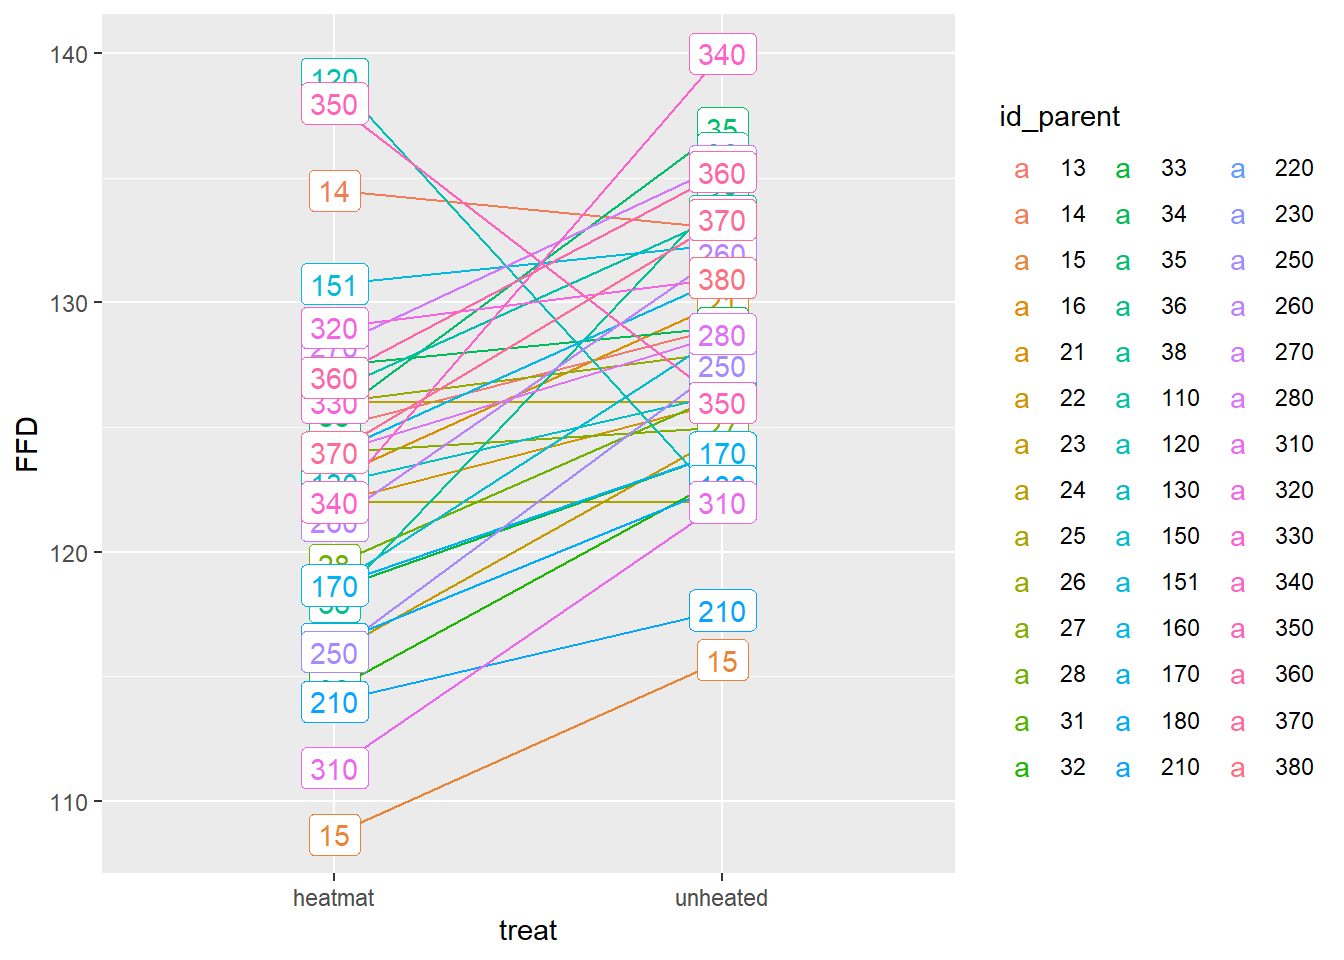
\includegraphics{1_data_prep_analyses_files/figure-latex/unnamed-chunk-15-1.pdf}

\begin{Shaded}
\begin{Highlighting}[]
\FunctionTok{plot}\NormalTok{(}\FunctionTok{ggpredict}\NormalTok{(model\_parents\_LFD,}\AttributeTok{terms=}\FunctionTok{c}\NormalTok{(}\StringTok{"treat"}\NormalTok{)))}
\end{Highlighting}
\end{Shaded}

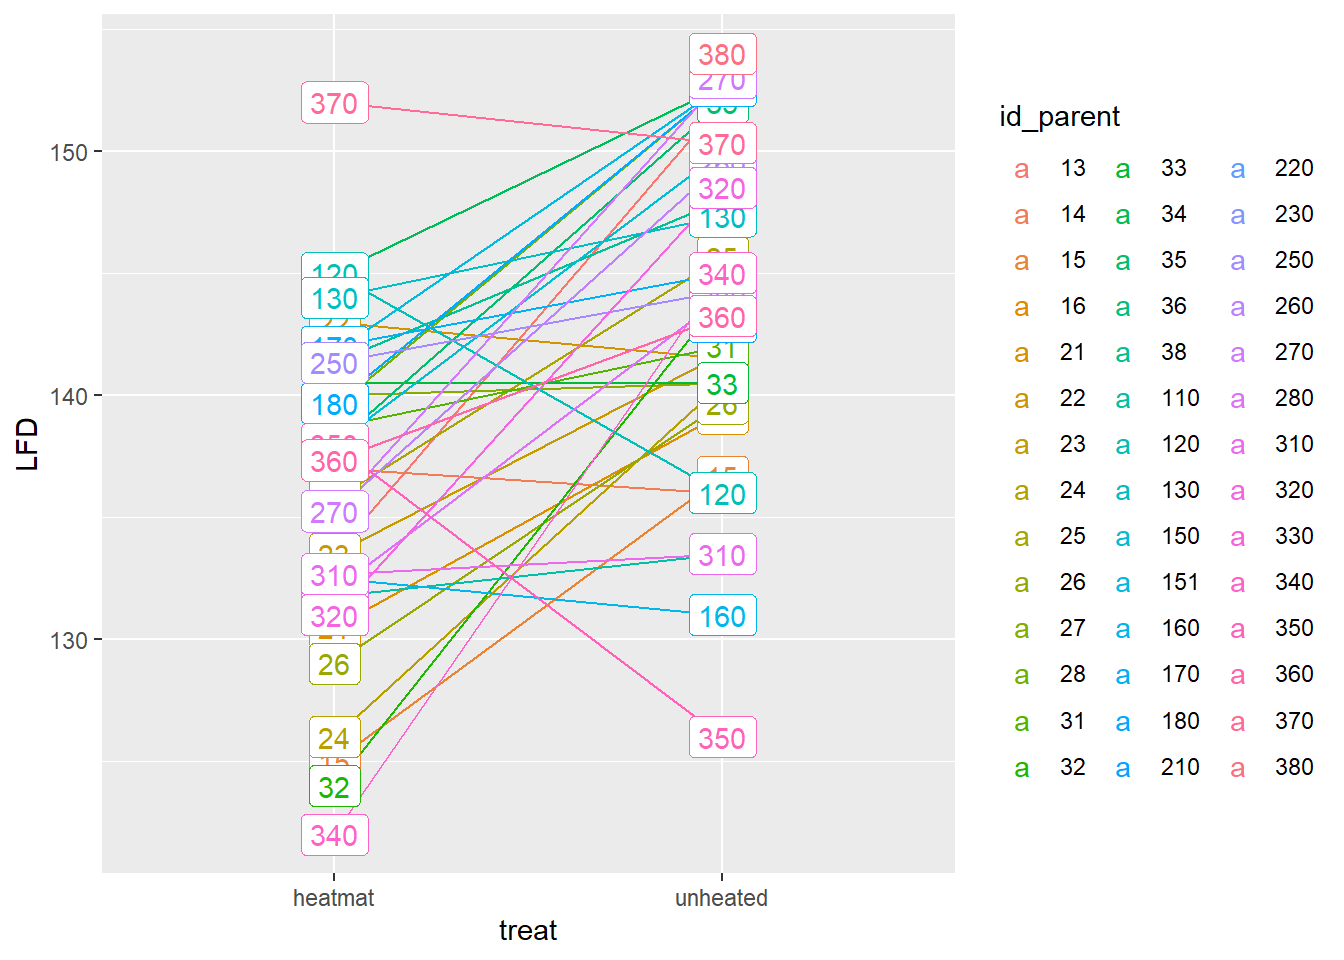
\includegraphics{1_data_prep_analyses_files/figure-latex/unnamed-chunk-15-2.pdf}

\begin{Shaded}
\begin{Highlighting}[]
\FunctionTok{plot}\NormalTok{(}\FunctionTok{ggpredict}\NormalTok{(model\_parents\_date50,}\AttributeTok{terms=}\FunctionTok{c}\NormalTok{(}\StringTok{"treat"}\NormalTok{)))}
\end{Highlighting}
\end{Shaded}

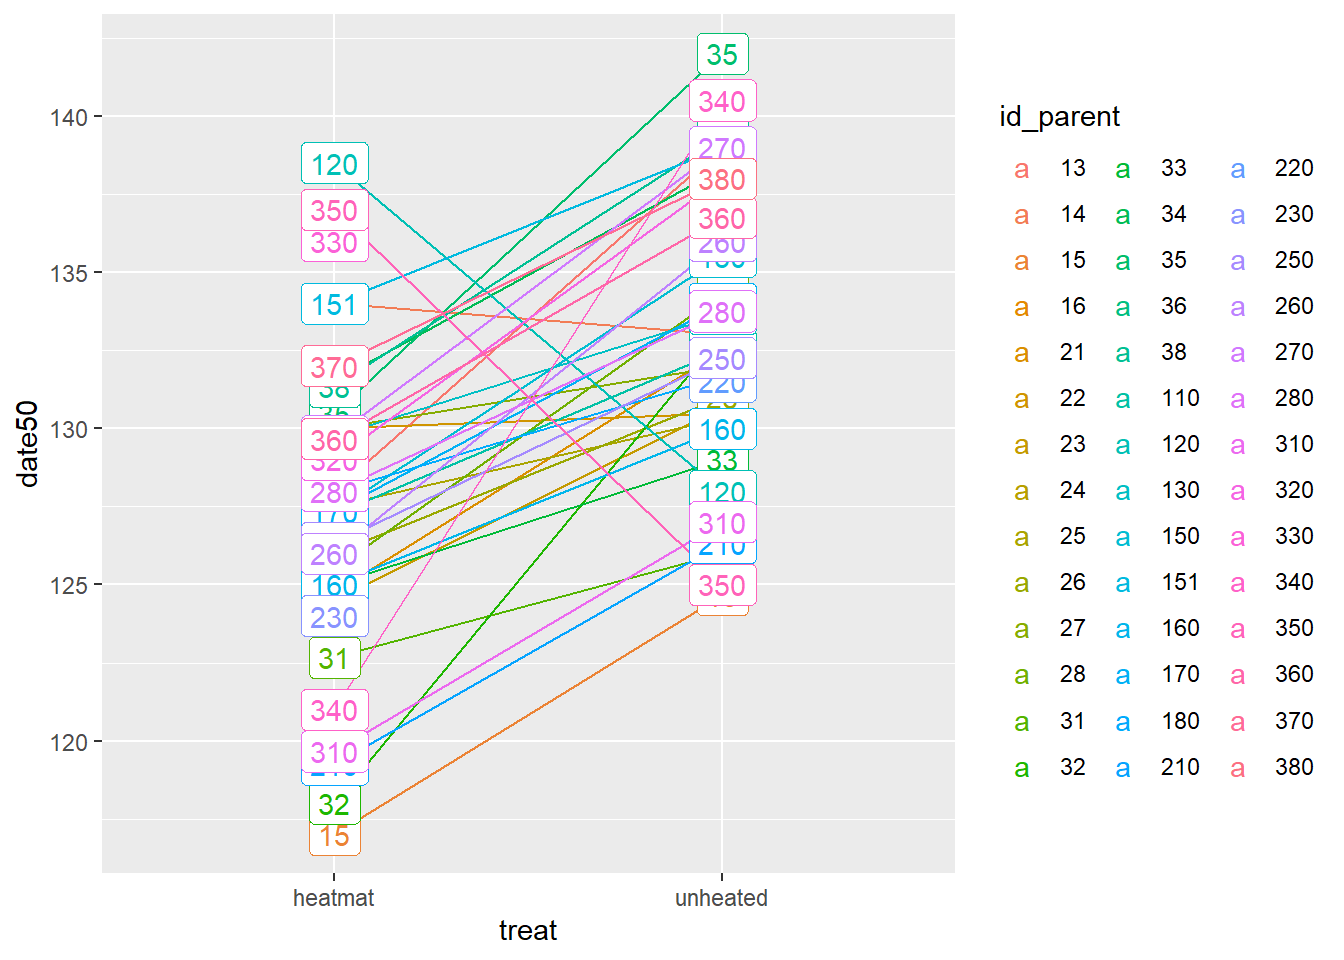
\includegraphics{1_data_prep_analyses_files/figure-latex/unnamed-chunk-15-3.pdf}

\begin{Shaded}
\begin{Highlighting}[]
\FunctionTok{plot}\NormalTok{(}\FunctionTok{ggpredict}\NormalTok{(model\_parents\_date50,}\AttributeTok{terms=}\FunctionTok{c}\NormalTok{(}\StringTok{"temp"}\NormalTok{)))}
\end{Highlighting}
\end{Shaded}

\includegraphics{1_data_prep_analyses_files/figure-latex/unnamed-chunk-15-4.pdf}

Plot predictions of interactions (NS)

\begin{Shaded}
\begin{Highlighting}[]
\FunctionTok{plot}\NormalTok{(}\FunctionTok{ggpredict}\NormalTok{(model\_parents\_FFD,}\AttributeTok{terms=}\FunctionTok{c}\NormalTok{(}\StringTok{"temp"}\NormalTok{,}\StringTok{"treat"}\NormalTok{)))}
\end{Highlighting}
\end{Shaded}

\includegraphics{1_data_prep_analyses_files/figure-latex/unnamed-chunk-16-1.pdf}

\begin{Shaded}
\begin{Highlighting}[]
\FunctionTok{plot}\NormalTok{(}\FunctionTok{ggpredict}\NormalTok{(model\_parents\_LFD,}\AttributeTok{terms=}\FunctionTok{c}\NormalTok{(}\StringTok{"temp"}\NormalTok{,}\StringTok{"treat"}\NormalTok{)))}
\end{Highlighting}
\end{Shaded}

\includegraphics{1_data_prep_analyses_files/figure-latex/unnamed-chunk-16-2.pdf}

\begin{Shaded}
\begin{Highlighting}[]
\FunctionTok{plot}\NormalTok{(}\FunctionTok{ggpredict}\NormalTok{(model\_parents\_date50,}\AttributeTok{terms=}\FunctionTok{c}\NormalTok{(}\StringTok{"temp"}\NormalTok{,}\StringTok{"treat"}\NormalTok{)))}
\end{Highlighting}
\end{Shaded}

\includegraphics{1_data_prep_analyses_files/figure-latex/unnamed-chunk-16-3.pdf}

\hypertarget{session-info}{%
\section{Session info}\label{session-info}}

\begin{Shaded}
\begin{Highlighting}[]
\FunctionTok{sessionInfo}\NormalTok{()}
\end{Highlighting}
\end{Shaded}

\begin{verbatim}
## R version 4.2.2 (2022-10-31 ucrt)
## Platform: x86_64-w64-mingw32/x64 (64-bit)
## Running under: Windows 10 x64 (build 22621)
## 
## Matrix products: default
## 
## locale:
## [1] LC_COLLATE=English_United States.utf8 
## [2] LC_CTYPE=English_United States.utf8   
## [3] LC_MONETARY=English_United States.utf8
## [4] LC_NUMERIC=C                          
## [5] LC_TIME=English_United States.utf8    
## 
## attached base packages:
## [1] stats     graphics  grDevices utils     datasets  methods   base     
## 
## other attached packages:
##  [1] knitr_1.42          broom.mixed_0.2.9.4 broom_1.0.3        
##  [4] jtools_2.2.1        sjPlot_2.8.12       car_3.1-1          
##  [7] carData_3.0-5       glmmTMB_1.1.5       ggeffects_1.2.0    
## [10] RColorBrewer_1.1-3  readxl_1.4.2        lubridate_1.9.2    
## [13] forcats_1.0.0       stringr_1.5.0       dplyr_1.1.0        
## [16] purrr_1.0.1         readr_2.1.4         tidyr_1.3.0        
## [19] tibble_3.1.8        ggplot2_3.4.1       tidyverse_2.0.0    
## 
## loaded via a namespace (and not attached):
##  [1] nlme_3.1-162        insight_0.19.0      numDeriv_2016.8-1.1
##  [4] tools_4.2.2         TMB_1.9.2           backports_1.4.1    
##  [7] utf8_1.2.3          R6_2.5.1            sjlabelled_1.2.0   
## [10] colorspace_2.1-0    withr_2.5.0         tidyselect_1.2.0   
## [13] emmeans_1.8.4-1     compiler_4.2.2      performance_0.10.2 
## [16] cli_3.6.0           sandwich_3.0-2      labeling_0.4.2     
## [19] bayestestR_0.13.0   scales_1.2.1        mvtnorm_1.1-3      
## [22] digest_0.6.31       minqa_1.2.5         rmarkdown_2.20     
## [25] pkgconfig_2.0.3     htmltools_0.5.4     parallelly_1.34.0  
## [28] lme4_1.1-31         highr_0.10          fastmap_1.1.1      
## [31] rlang_1.0.6         rstudioapi_0.14     farver_2.1.1       
## [34] generics_0.1.3      zoo_1.8-11          magrittr_2.0.3     
## [37] parameters_0.20.2   Matrix_1.5-3        Rcpp_1.0.10        
## [40] munsell_0.5.0       fansi_1.0.4         abind_1.4-5        
## [43] lifecycle_1.0.3     furrr_0.3.1         stringi_1.7.12     
## [46] multcomp_1.4-22     yaml_2.3.7          MASS_7.3-58.2      
## [49] grid_4.2.2          parallel_4.2.2      listenv_0.9.0      
## [52] sjmisc_2.8.9        crayon_1.5.2        lattice_0.20-45    
## [55] haven_2.5.2         splines_4.2.2       pander_0.6.5       
## [58] sjstats_0.18.2      hms_1.1.2           pillar_1.8.1       
## [61] boot_1.3-28.1       estimability_1.4.1  effectsize_0.8.3   
## [64] codetools_0.2-19    glue_1.6.2          evaluate_0.20      
## [67] modelr_0.1.10       vctrs_0.5.2         nloptr_2.0.3       
## [70] tzdb_0.3.0          cellranger_1.1.0    gtable_0.3.1       
## [73] future_1.31.0       datawizard_0.6.5    xfun_0.37          
## [76] xtable_1.8-4        coda_0.19-4         survival_3.5-3     
## [79] timechange_0.2.0    globals_0.16.2      TH.data_1.1-1      
## [82] ellipsis_0.3.2
\end{verbatim}

\end{document}
